\clearpage\section*{Post hoc external output diagnostics}

The 12 October 2026 addendum was written before these computations, but after the external outcomes were known. No fitting, peak selection or new inferential test was performed. Exports include all 36 frozen states and both populations. The displays below show all three selected Swin Soft/Uniform seeds, not only favorable ones.

\begin{table}[H]
\caption{Principal selected Swin predicted-category proportions at 80\% MSP (\%). Columns retain every seed; each contains 1,152 clips}\label{tab:externalcategories}
\centering\small\begin{tabular}{lrrrrrr}\toprule
 & \multicolumn{3}{c}{Soft} & \multicolumn{3}{c}{Uniform}\\
Category & 17 & 42 & 89 & 17 & 42 & 89\\\midrule
Angry & 0.87 & 1.13 & 1.22 & 1.48 & 1.74 & 1.22\\
Disgust & 0.35 & 0.00 & 0.09 & 0.61 & 0.17 & 0.00\\
Fear & 0.00 & 0.00 & 0.00 & 0.00 & 0.00 & 0.00\\
Happy & 23.96 & 23.18 & 23.70 & 26.74 & 24.57 & 22.92\\
Neutral & 68.14 & 69.97 & 67.01 & 64.58 & 62.67 & 68.32\\
Sad & 3.04 & 2.78 & 3.65 & 3.04 & 5.56 & 3.30\\
Surprise & 3.65 & 2.95 & 4.34 & 3.56 & 5.30 & 4.25\\
\bottomrule\end{tabular}\end{table}

Across all 1,440 clips, raw human-vote mass (\%) is angry: 14.46, disgust: 11.66, fear: 11.21, happy: 16.77, neutral: 9.06, sad: 14.21, surprise: 10.74, calm: 8.76, none: 3.14. Accepted-set vote masses are exported separately for every state and seed; model counts and reference vote mass are distinct quantities.

\begin{figure}[H]\centering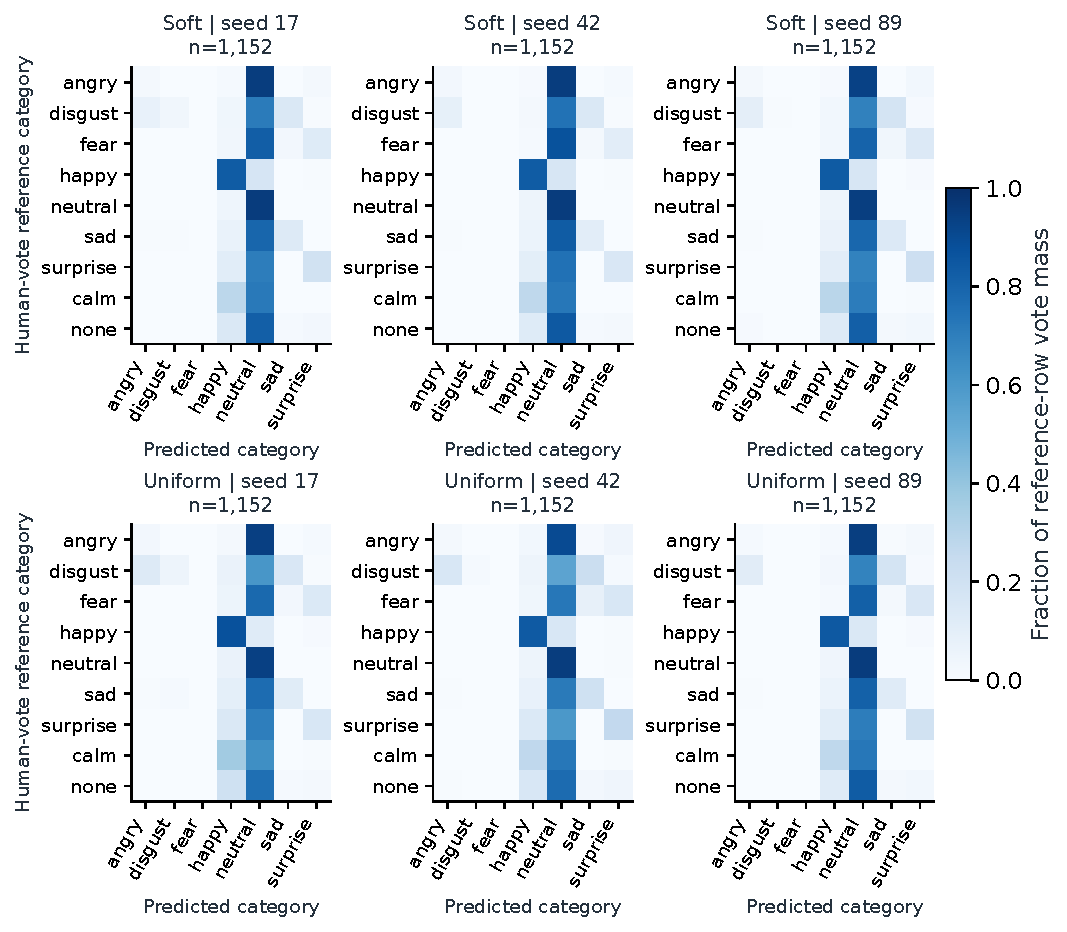
\includegraphics[width=\linewidth]{submission_reader_2026_10_13/source/figures/ExternalVoteMatrices.pdf}

\caption{Human-vote reference versus predicted category for all principal selected Swin Soft/Uniform seeds at 80\% MSP. Each cell divides the vote mass assigned to that predicted column by the row total; it is not single-label confusion or frame accuracy. Calm and none rows remain although the model has no corresponding outputs. Every panel contains 1,152 clips. All 36 states, both populations, raw contributions, row masses and both references are in Online Resource 8. Rows with no vote mass are undefined, not zero. The common scale is 0--1}\end{figure}

\clearpage\begin{figure}[H]\centering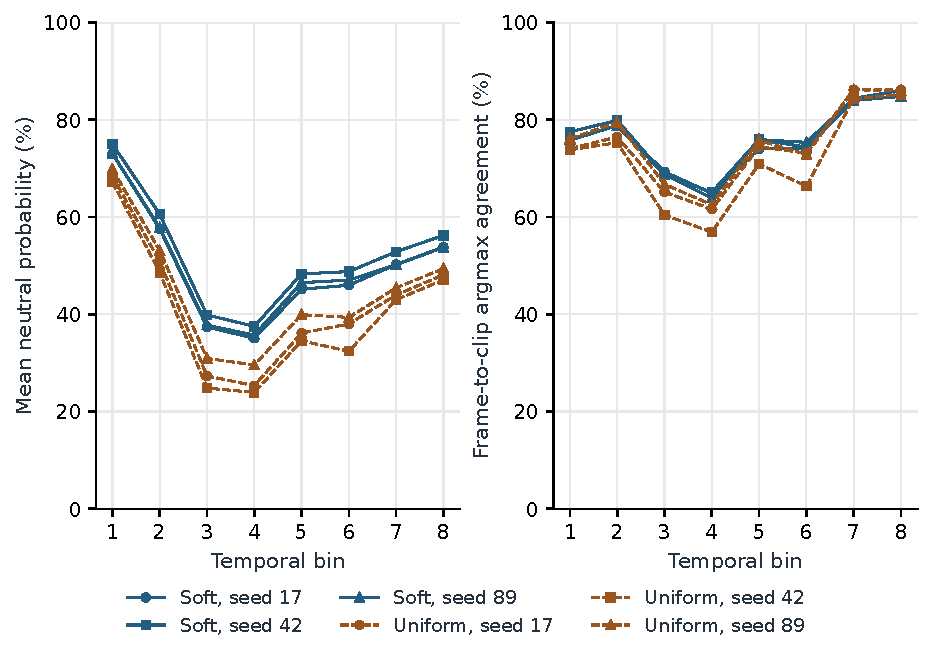
\includegraphics[width=\linewidth]{submission_reader_2026_10_13/source/figures/ExternalTemporal.pdf}

\caption{Predictions across all eight temporal bins for selected Swin Soft/Uniform and all three seeds. Left: mean neutral probability. Right: agreement between frame-level and mean-probability clip predictions from the same model. Each bin has 1,440 valid frames from 1,440 clips; each state has 11,520 frames. Human judgments are clip-level, so agreement is not frame accuracy. Exports include all categories and all 36 states. Temporal patterns do not establish why external disagreement occurs}\end{figure}

Acquisition checks verify video-only speech IDs, ten responses per clip, primary response mapping, frame-bin indices, shared crop validity and canonical category order. Every clip has eight valid frames. Independently summing retained float32 frame probabilities in float64 reproduces the clip mean exactly (maximum absolute difference zero). Raw/merged scoring preserves predictions and accepted IDs. Diagnostic identities use tolerance $10^{-10}$ for vote-mass summation and $10^{-14}$ for clip aggregation; probability normalization tolerance is $10^{-6}$.
